% !TeX spellcheck = es_MX
\documentclass[12pt, a4paper, titlepage]{article}
\usepackage[spanish]{babel}
\usepackage[utf8]{inputenc}
\usepackage[linesnumbered,lined,boxed,commentsnumbered]{algorithm2e}
\usepackage{enumitem,kantlipsum}
\usepackage{array}
\usepackage{placeins}
% Códigos y codificación para caracteres en español
\usepackage{listings}
\usepackage{color}
\lstset{literate=
	{á}{{\'a}}1 {é}{{\'e}}1 {í}{{\'i}}1 {ó}{{\'o}}1 {ú}{{\'u}}1
	{Á}{{\'A}}1 {É}{{\'E}}1 {Í}{{\'I}}1 {Ó}{{\'O}}1 {Ú}{{\'U}}1
	{à}{{\`a}}1 {è}{{\`e}}1 {ì}{{\`i}}1 {ò}{{\`o}}1 {ù}{{\`u}}1
	{À}{{\`A}}1 {È}{{\'E}}1 {Ì}{{\`I}}1 {Ò}{{\`O}}1 {Ù}{{\`U}}1
	{ä}{{\"a}}1 {ë}{{\"e}}1 {ï}{{\"i}}1 {ö}{{\"o}}1 {ü}{{\"u}}1
	{Ä}{{\"A}}1 {Ë}{{\"E}}1 {Ï}{{\"I}}1 {Ö}{{\"O}}1 {Ü}{{\"U}}1
	{â}{{\^a}}1 {ê}{{\^e}}1 {î}{{\^i}}1 {ô}{{\^o}}1 {û}{{\^u}}1
	{Â}{{\^A}}1 {Ê}{{\^E}}1 {Î}{{\^I}}1 {Ô}{{\^O}}1 {Û}{{\^U}}1
	{œ}{{\oe}}1 {Œ}{{\OE}}1 {æ}{{\ae}}1 {Æ}{{\AE}}1 {ß}{{\ss}}1
	{ű}{{\H{u}}}1 {Ű}{{\H{U}}}1 {ő}{{\H{o}}}1 {Ő}{{\H{O}}}1
	{ç}{{\c c}}1 {Ç}{{\c C}}1 {ø}{{\o}}1 {å}{{\r a}}1 {Å}{{\r A}}1
	{€}{{\EUR}}1 {£}{{\pounds}}1
}

%%Appendix
\usepackage[toc,page]{appendix}

%%otros
\usepackage{float}
\usepackage{subfig}
\usepackage{comment}

% http://ctan.org/pkg/booktabs
\usepackage{booktabs}
\newcommand{\tabitem}{~~\llap{\textbullet}~~}

%%Imágenes
\usepackage{graphicx}

%%Colores de texto 
\usepackage{xcolor}
\usepackage{colortbl}

%%Links
\usepackage[hidelinks]{hyperref}

%%Comentarios
\usepackage{verbatim}

%%PARA IMÁGENES EN LÍNEA
%\usepackage[english]{babel}

\usepackage{pdfpages}

%------------------------------------------------ESTABLECER COLORES------------------------------------------------%

\definecolor{guindapoli}{RGB}{102, 0, 51}
\definecolor{azulescom}{RGB}{0, 0, 102}
\definecolor{azulclaro}{RGB}{222, 232, 255}
\definecolor{azulfuerte}{RGB}{60, 150, 250}

%------------------------------------------------FIN DE COLORES------------------------------------------------%


\begin{document}
	%%PARA QUE DETECTE HASTA SUBSUBSECTION
	\setcounter{secnumdepth}{3}
	
	%%%%%%%%%%%%%%%%%%%%%%%%%%%%%%%%%%%%%%%%%%%%%%%%%%%%%%%%%
	%                                                       																																		  %
	%                                                      																																	  		  %
	%              																	PORTADA  																				  			 %
	%                                                      																																			  %
	%                                                      																																			  %
	%%%%%%%%%%%%%%%%%%%%%%%%%%%%%%%%%%%%%%%%%%%%%%%%%%%%%%%%%
	\begin{titlepage}	
		
		\newcommand{\HRule}{\rule{\linewidth}{0.5mm}}									%%%\left
		%%%
		\begin{minipage}{0.46\textwidth} \begin{flushleft}
				
\includegraphics[scale = 0.10]{Imagenes/Logos/logoescom.png}
		\end{flushleft}\end{minipage}
		\begin{minipage}{0.48\textwidth} \begin{flushright}
				
\includegraphics[scale = 0.55]{Imagenes/Logos/logoipn.png}
		\end{flushright}\end{minipage}
		
		%%%
		\vspace*{.25cm}								%%%
		
		\begin{center}
			
			\begin{LARGE}
				\textcolor{guindapoli}{INSTITUTO POLITÉCNICO NACIONAL}\\
			\end{LARGE}	
			
			\vspace*{0.2in}
			
			\begin{Large}
				\textcolor{azulescom}{ESCUELA SUPERIOR DE CÓMPUTO}\\
			\end{Large}	
		
			\vspace*{0.4in}
			
			\begin{large}
				Manual de Usuario\\
			\end{large}	
			
			\vspace*{0.4in}
			
			\begin{large}
			TT 2020-B002\\
			\end{large}
			
			\vspace*{0.2in}
			
			\begin{Large}
				\textbf{Generador de versos musicales en el idioma
					inglés por medio de procesamiento de lenguaje
					natural y redes neuronales}\\
			\end{Large}
						
			\vspace*{0.2in}
			
			\rule{80mm}{.1mm}\\
			\vspace*{0.1in}
			
			\begin{large}
				\begin{center}
					\textbf{Presentan}:\\
					Espinosa de los Monteros Lechuga Jaime Daniel\\
					Nava Romo Edgar Adrián\\
					Salgado Gómez Alfredo Emilio\\
				\end{center}
			\end{large}
			
			\begin{large}
				\textbf{Directores}:\\
				Olga Kolesnikova\\
				Ariel López Rojas\\
			\end{large}
			
		\end{center}
		
	\end{titlepage}
	
	%%%%%%%%%%%%%%%%%%%%%%%%%%%%%%%%%%%%%%%%%%%%%%%%%%%%%%%%%
	%                                                       																																		  %
	%                                                      																																	  		  %
	%              																	 ÍNDICE  																				  			 	  %
	%                                                      																																			  %
	%                                                      																																			  %
	%%%%%%%%%%%%%%%%%%%%%%%%%%%%%%%%%%%%%%%%%%%%%%%%%%%%%%%%%
	% Firma directores
	\newpage
	% Rename Appendice to Anexos
	\renewcommand\appendixpagename{Índice}
	\renewcommand\appendixtocname{Índice}
	\appendixpageoff
	\begin{appendices}
		\renewcommand*\contentsname{{\textcolor{azulescom}{Índice.}}}
		\tableofcontents
		\newpage
		%%índice de figuras
		\renewcommand*\listfigurename{{\textcolor{azulescom}{Índice de figuras.}}}
		\listoffigures
		\newpage
		%%Índice de tablas
		\newpage
	\end{appendices}
	
	\section{Introducción}
	El siguiente manual muestra los pasos a seguir para aprovechar
	en su mayor capacidad la aplicación web la cual permite al usuario
	generar letras musicales a partir de ciertos parámetros proporcionados
	por el usuario. Con la finalidad de brindar al usuario una herramienta
	que le asegure el uso correcto de la aplicación web.
	
	\section{Requerimientos}
	En esta sección se enumeran los requisitos de hardware y
	software de las aplicaciones basadas en modelo y
	aplicaciones cliente para dispositivos móviles.
	
		\subsection{Requisitos de hardware de aplicaciones web}
			En la tabla siguiente se enumeran los requisitos
			de hardware mínimos y recomendados para la aplicación web.
		
			\begin{table}[!htbp]
				\caption[Requisitos hardware]{Requisitos de hardware mínimos y recomendados}
				\begin{tabular}{| p{4cm} | p{4cm} | p{4cm} |} 
					\hline
					\textbf{Componente} & \textbf{Mínimo} & \textbf{Recomendado} \\ 
					\hline
					Procesador & Procesador de x86 o x64 bits de doble núcleo de 1,9 gigahercios (GHz) o más con el conjunto de instrucciones SSE2 & Procesador de 64 bits de doble núcleo de 3,3 gigahercios (GHz) o más con el conjunto de instrucciones SSE2 \\ 
					\hline
					Memoria & 2 GB de RAM & 4 GB de RAM o más \\
					\hline
					Resolución  & Súper VGA con una resolución de 1024 x 768 & Súper VGA con una resolución de 1024 x 768 \\
					\hline
				\end{tabular}
			\end{table}
		
			
			La ejecución de aplicaciones basadas en modelo en un equipo
			que no cumpla los requisitos recomendados puede producir un
			rendimiento inadecuado. Además, puede experimentarse
			rendimiento satisfactorio ejecutando sistemas que usan otra
			configuración de hardware que los publicados aquí.\\\\
			Por ejemplo, un sistema con un procesador moderno
			de cuatro núcleos, velocidad de reloj más baja y más RAM.
		
		\subsection{Requisitos de red}
		Las aplicaciones basadas en modelo están diseñadas para funcionar
		mejor en redes que tienen los siguientes elementos:
		
		\begin{itemize}
			\item Ancho de banda superior a 50 KBps (400 kbps)
			\item Latencia inferior a 150 ms
		\end{itemize}
		
		Tenga en cuenta que estos valores son recomendaciones y no garantizan
		un rendimiento satisfactorio. Los valores recomendados se basan en los
		sistemas que usan solicitudes de un formulario con palabras usuales,
		el resultado podría variar.
		
		\subsection{Exploradores web admitidos}
			La aplicación web puede ejecutarse en cualquiera de los siguientes
			exploradores web que se ejecutan en los sistemas operativos especificados:
			\begin{itemize}
			\item Microsoft Edge (última versión lanzada públicamente) que se ejecuta en Windows 10, Windows 8.1, Windows 8, Windows 7
			\item Mozilla Firefox (última versión lanzada públicamente) que se ejecuta en Windows 10, Windows 8.1, Windows 8 o Windows 7
			\item Google Chrome (última versión lanzada públicamente) que se ejecuta en Windows 10, Windows 8.1, Windows 8, Windows 7
			\item Google Chrome (última versión de lanzamiento público) que se ejecuta en las dos últimas versiones de Mac OS de lanzamiento público
			\item Apple Safari (última versión de lanzamiento público) que se ejecuta en las dos últimas versiones de Mac OS de lanzamiento público o Apple iPad
			\end{itemize}
			
			Para buscar la última versión para estos exploradores web,
			visite el sitio web del fabricante del software.
	
	\newpage
	
	\section{Acceso a la aplicación web}
	Una vez ingresando al sitio web \textbf{www.neuralyrics.com} y este termine
	de desplegarse, se podrá empezar a interactuar en la misma.\\\\
		\begin{figure}[H]
		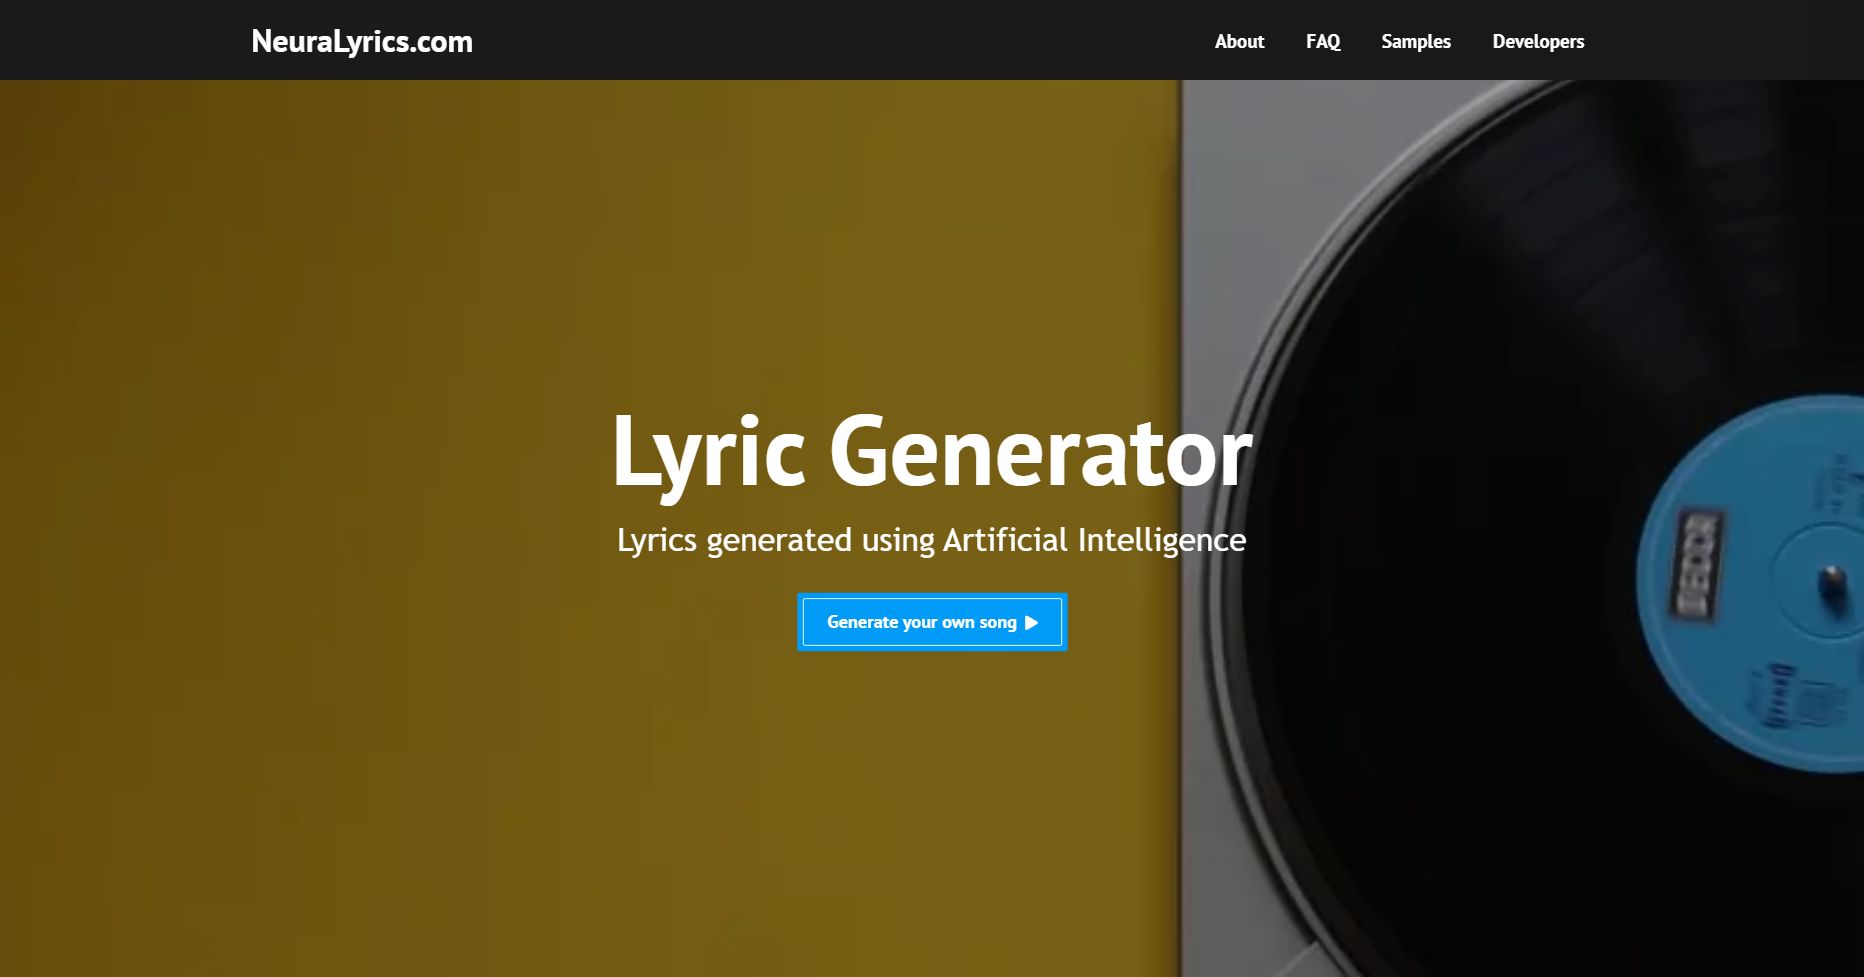
\includegraphics[width=13.5cm]{./Imagenes/Capturas/pprincipal.png}
		\centering \caption{Pantalla principal al terminar la carga.}
	\end{figure}

	\section{Barra de accesos}
	La barra de accesos cuenta con el título de todas las pantallas disponibles del sitio donde el usuario podrá interactuar con cada una de ellas y tiene un indicador de la pantalla activa para mayor comodidad visual.\\\\
	Si el usuario da clic en cualquier momento al logo de la página podrá regresar al inicio de todo el sitio web.\\\\
	Esta barra de herramientas aparece en todas las pantallas para que sea posible el fácil acceso a cualquier pantalla.
	
	\begin{figure}[H]
		
\includegraphics[width=13.5cm]{./Imagenes/Capturas/pbarra.png}
		\centering \caption{Barra de accesos disponibles para el usuario.}
	\end{figure}
	\begin{itemize}
		\item Home
		\item About
		\item Samples
		\item Contact
		\item Team
		\item FAQ
		\item Developers
	\end{itemize}
	\section{Página principal}
	Al entrar, se muestra la siguiente pantalla donde se muestran dos leyendas breves y un botón invitando a empezar el funcionamiento principal de la aplicación web.
	\begin{figure}[H] 
		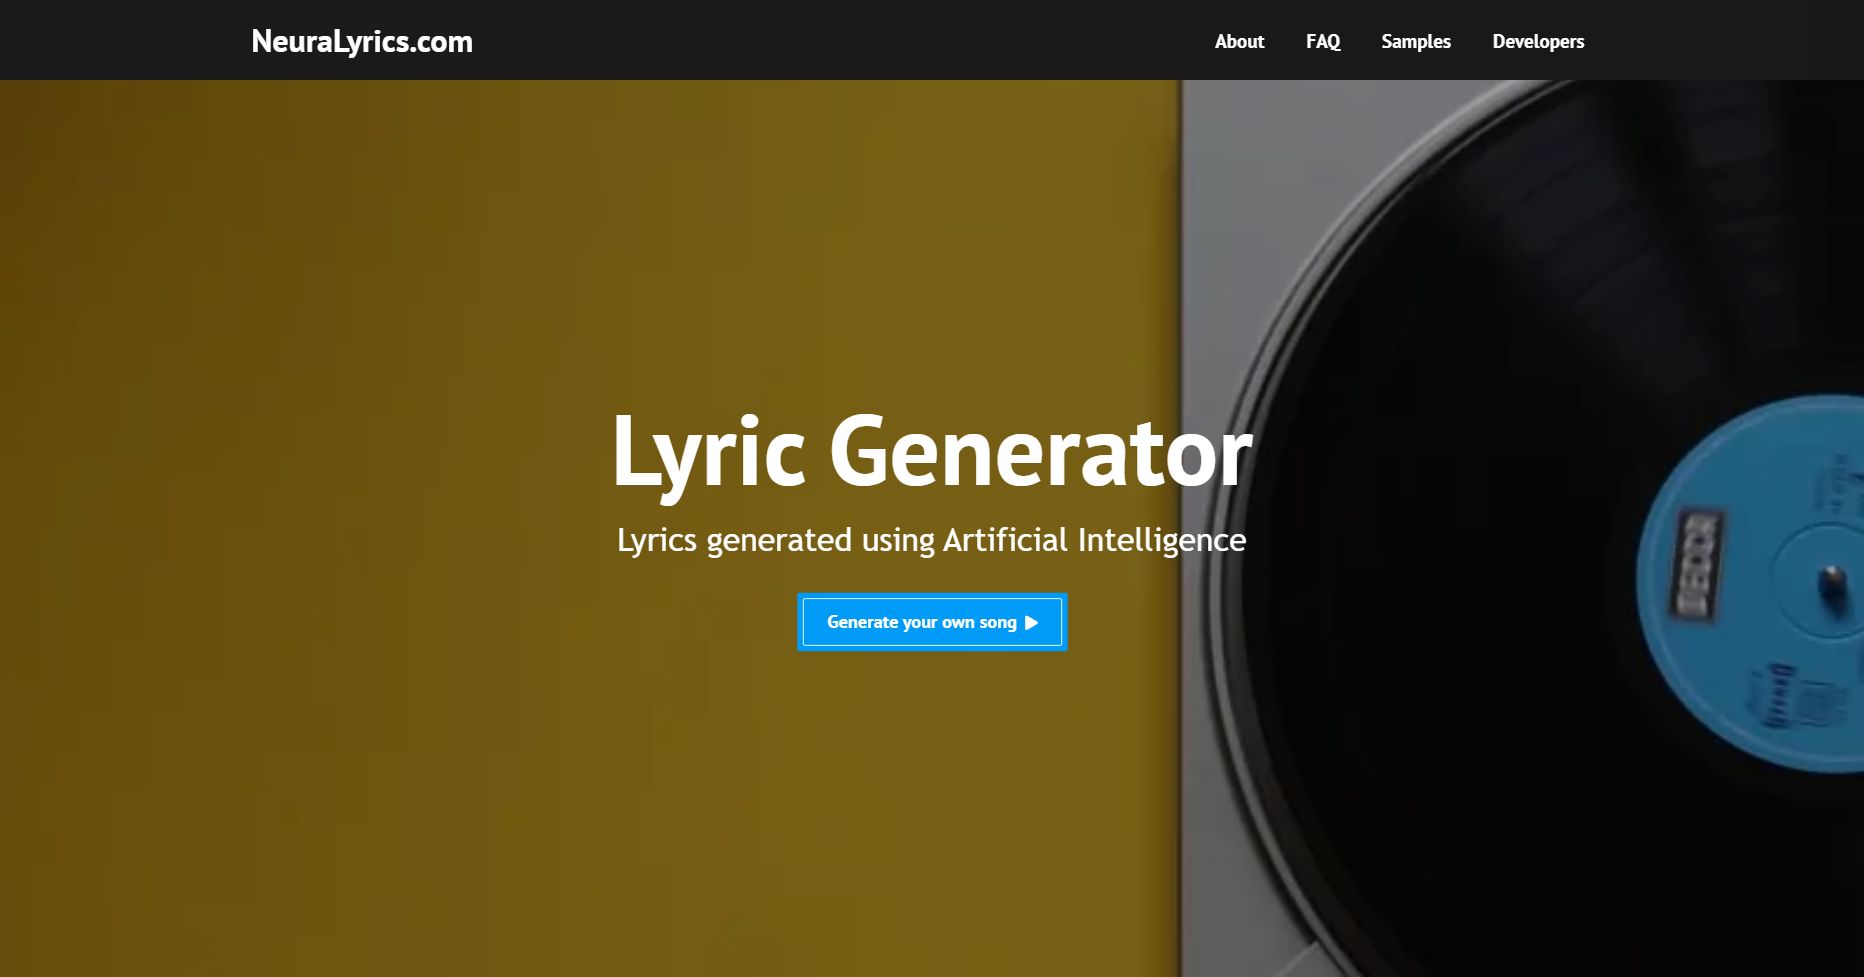
\includegraphics[width=13.5cm]{./Imagenes/Capturas/pprincipal.png}
		\centering \caption{Página de inicio de la aplicación web.}
	\end{figure}
	\subsection{Inicio de la generación de letras de canciones}
		Si se da clic al botón mencionado anteriormente, se va a iniciar un efecto de desvanecimiento del texto de toda la pantalla para iniciar otro efecto para que aparezcan nuevas instrucciones en esta misma pantalla, todo esto sin necesidad de otra interacción, esto con el objetivo de que las distracciones se eliminen completamente y se pueda concentrar en el funcionamiento de la aplicación.
		\begin{figure}[H] 
			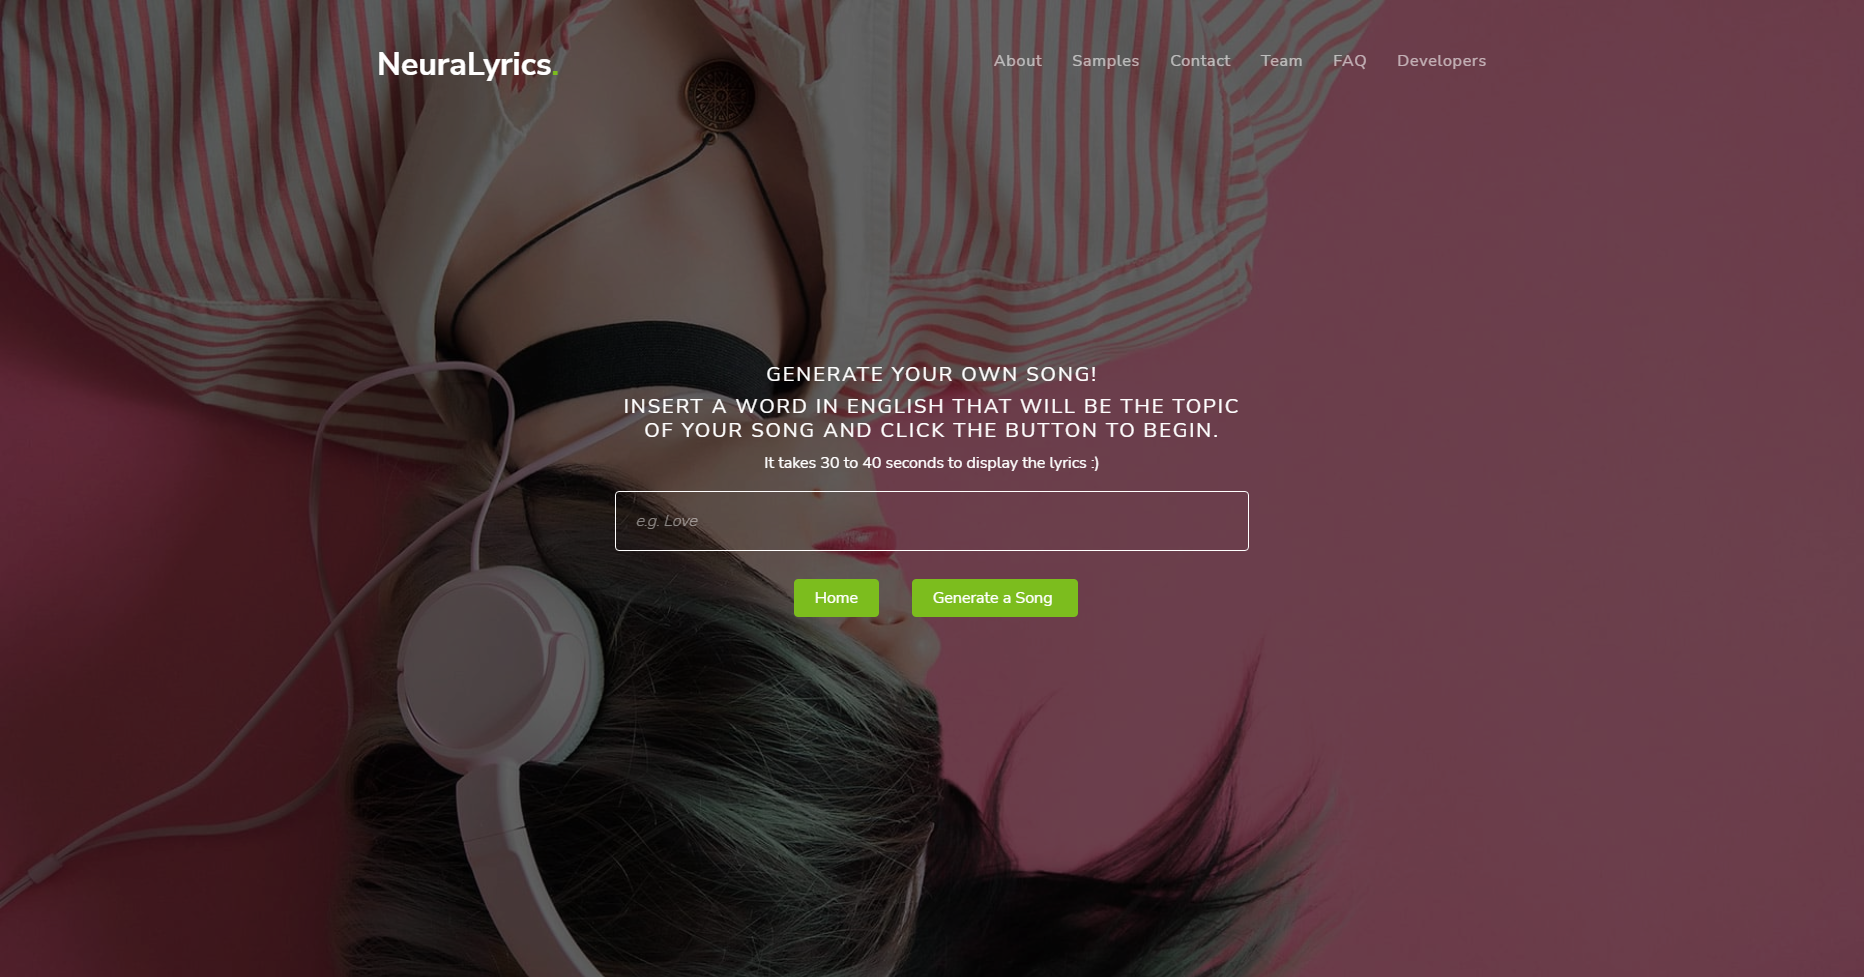
\includegraphics[width=13.5cm]{./Imagenes/Capturas/pform.png}
			\centering \caption{Segunda pantalla al dar clic al botón principal.}
		\end{figure}
	\subsection{Segunda pantalla para generar letras de canciones}
	La siguiente pantalla después del desvanecimiento, muestra instrucciones para ingresar una palabra en idioma inglés dentro de un campo vacío, así como un botón para empezar a generar la letra musical.
	\begin{figure}[H] 
		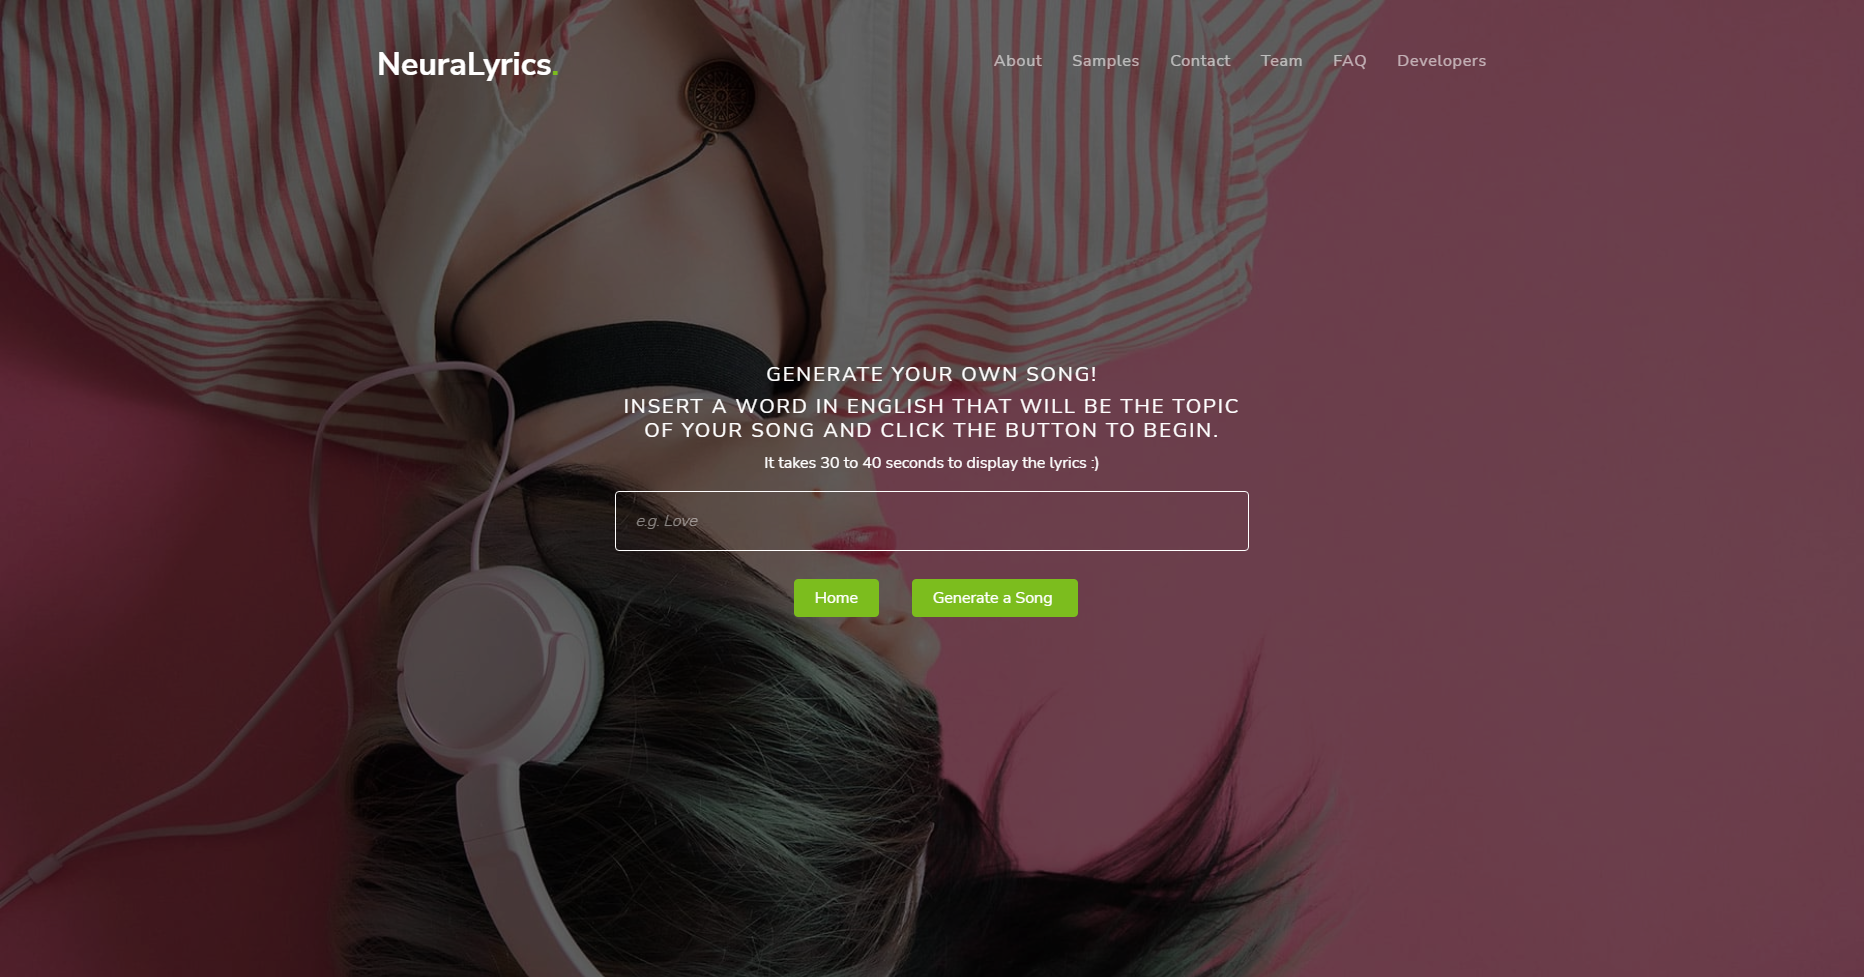
\includegraphics[width=13.5cm]{./Imagenes/Capturas/pform.png}
		\centering \caption{Página del funcionamiento para generar una letra de canción.}
	\end{figure}
	
	Si el campo se deja vacío y se da clic al botón para generar una canción, se mostrará un mensaje obligando a rellenar el campo.
	
	\begin{figure}[H] 
		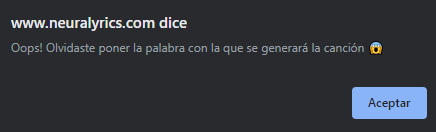
\includegraphics[width=13.5cm]{./Imagenes/Capturas/Noword.png}
		\centering \caption{Mensaje mostrado si el campo se dejó vacío.}
	\end{figure}
	\subsection{Resultado mostrando la letra de canción}
	En caso que se de clic al botón cumpliendo los requerimientos presentados en las instrucciones, se seguirá a una pantalla de carga en lo que se procesa la solicitud al sistema central de la aplicación.
	
	\begin{figure}[H] 
		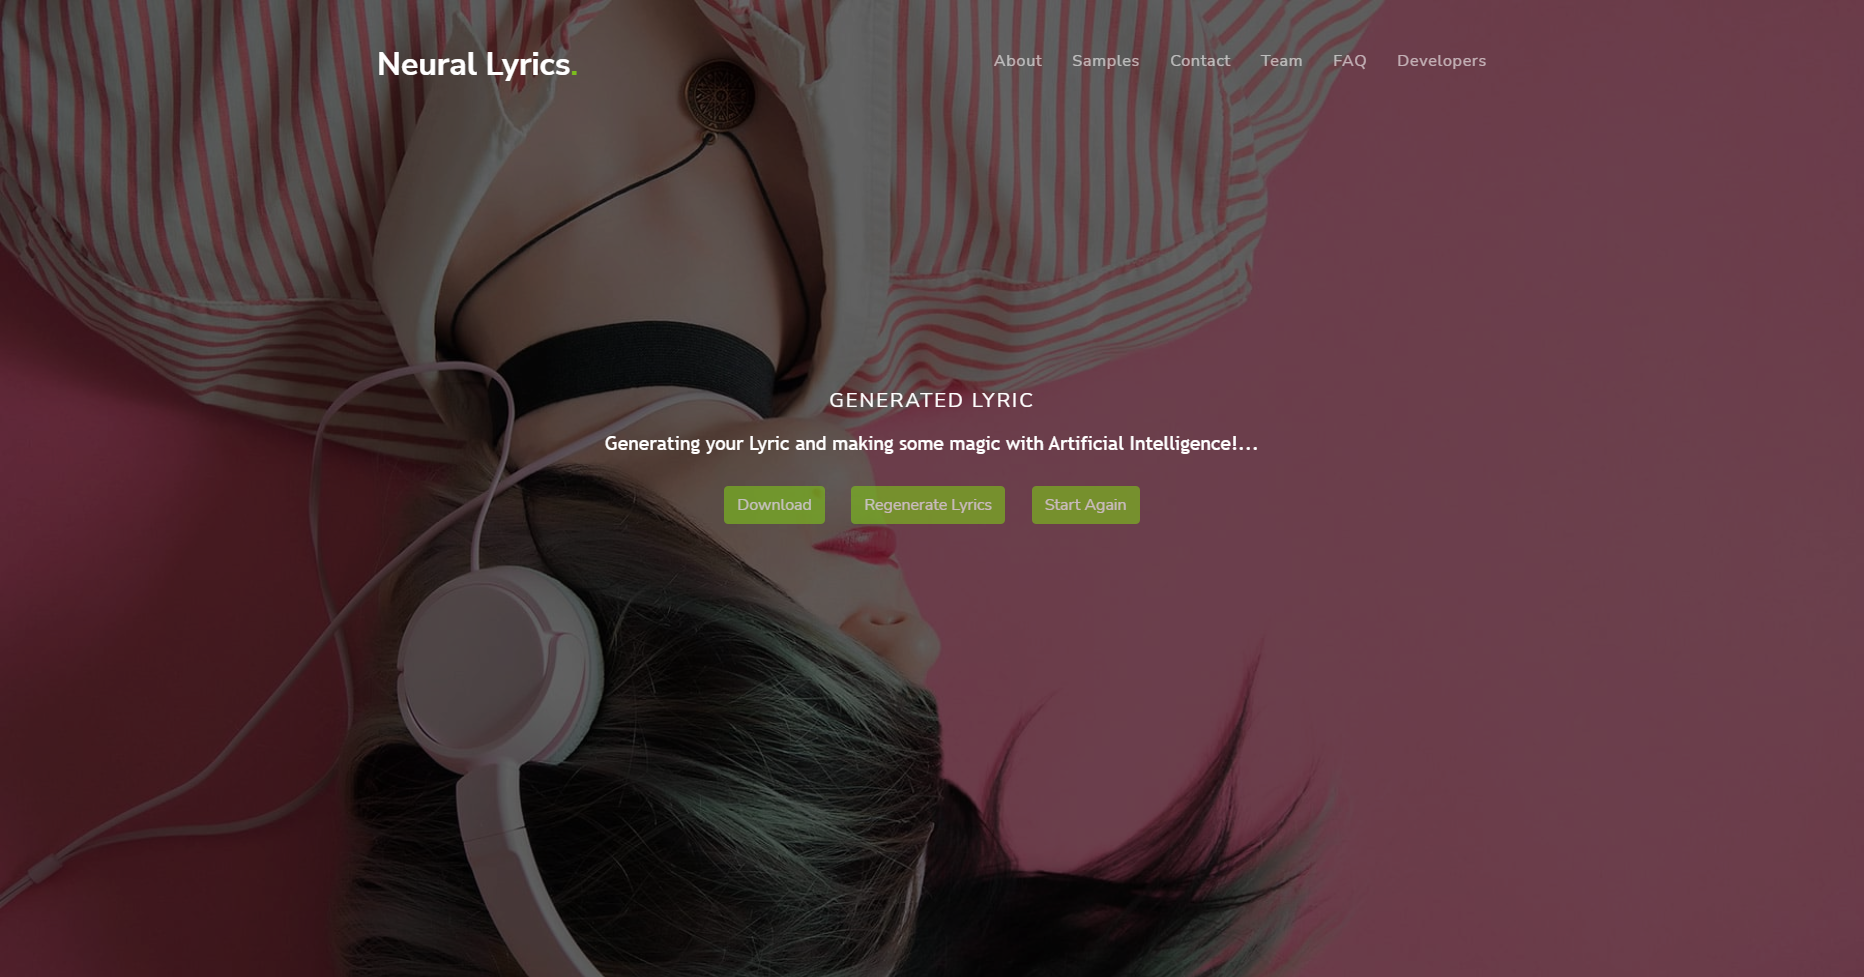
\includegraphics[width=13.5cm]{./Imagenes/Capturas/pgenerating.png}
		\centering \caption{Pantalla de carga.}
	\end{figure}
	Dentro de esta pantalla de carga se desplegarán al usuario datos curiosos relacionados con la música, esto con el fin de hacerle más amena la espera al usuario en lo que se está genera la letra.
	\begin{figure}[H] 
		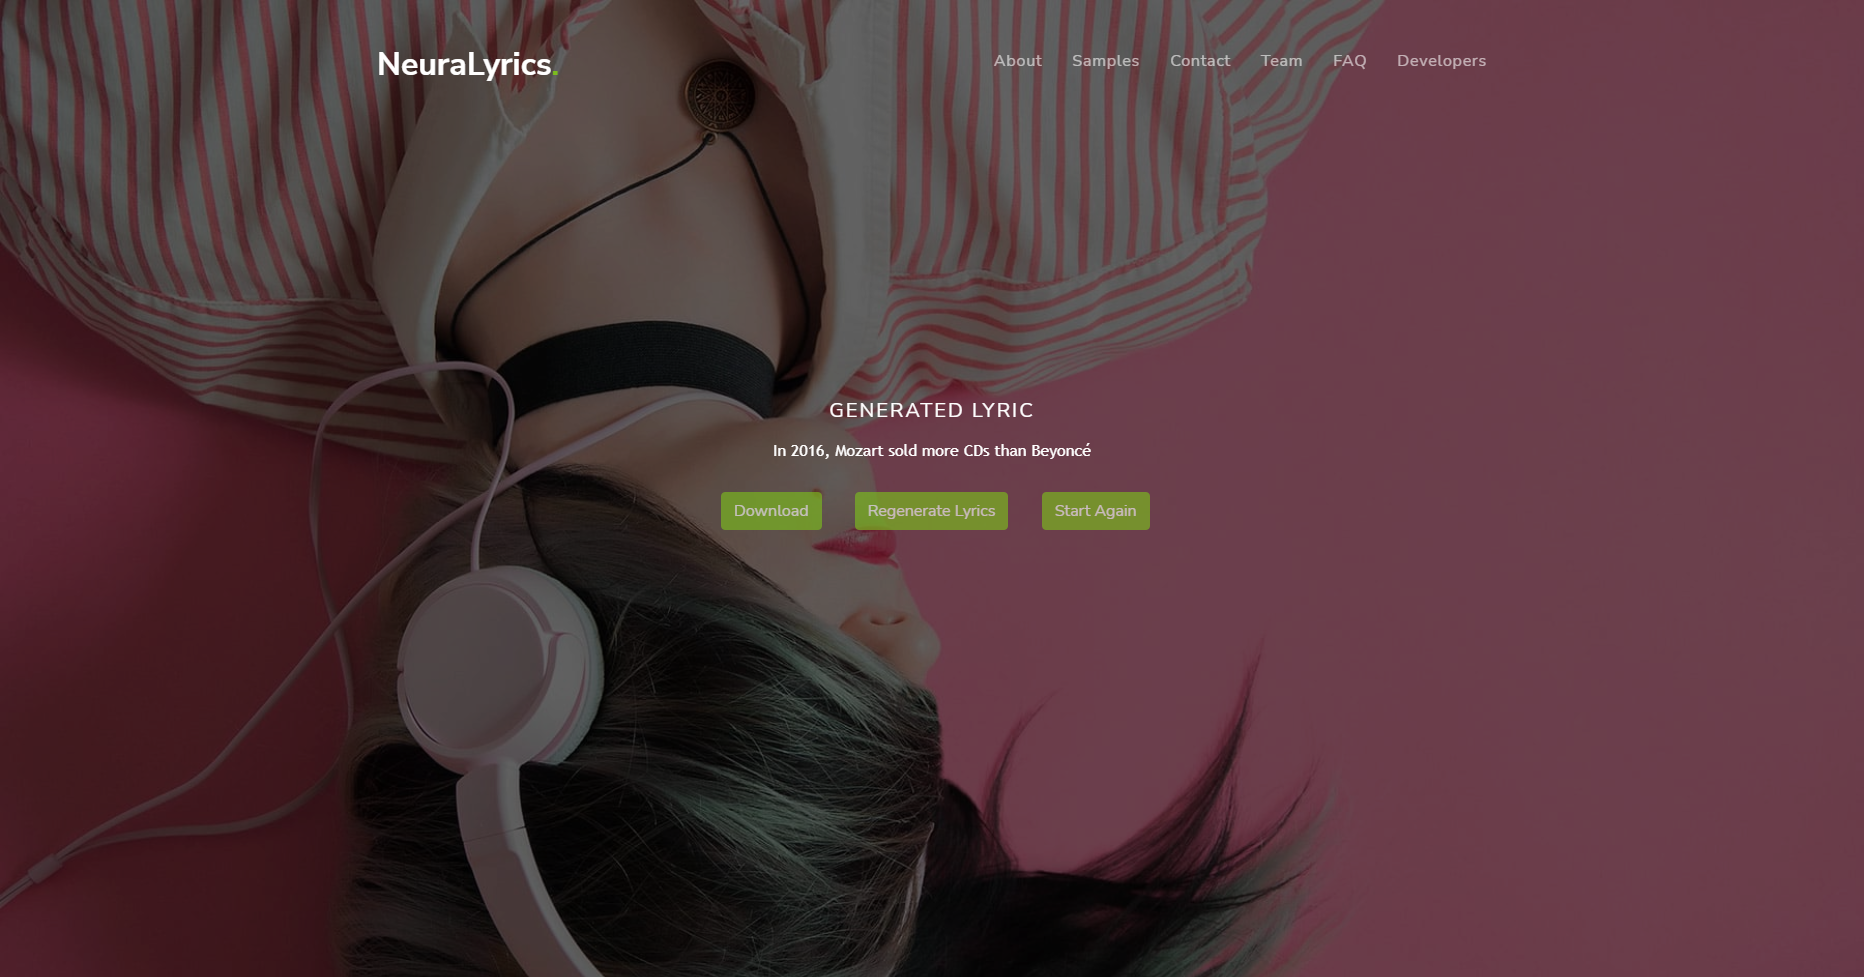
\includegraphics[width=13.5cm]{./Imagenes/Capturas/ffact.png}
		\centering \caption{Pantalla de carga con un dato curioso.}
	\end{figure}
	Una vez procesada la solicitud, se empezará a generar la canción con un efecto de typewriter dando como resultado final la letra de la canción final con tres botones diferentes, mientras se esta generando la letra, estos botones se encontraran bloqueados:
	\begin{itemize}
		\item Download: Descarga la canción en formato txt.
		
		\begin{figure}[H] 
			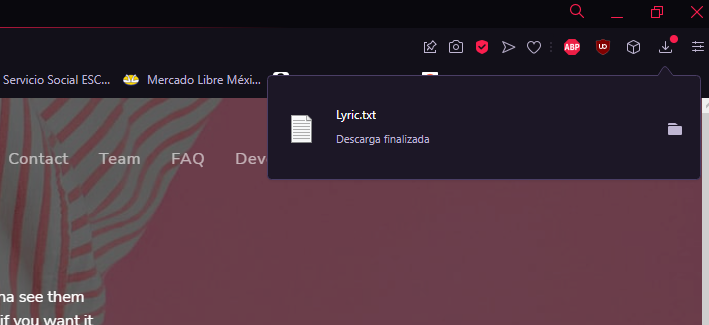
\includegraphics[width=13.5cm]{./Imagenes/Capturas/Download.png}
			\centering \caption{Botón de descarga en funcionamiento.}
		\end{figure}
	
		\begin{figure}[H] 
			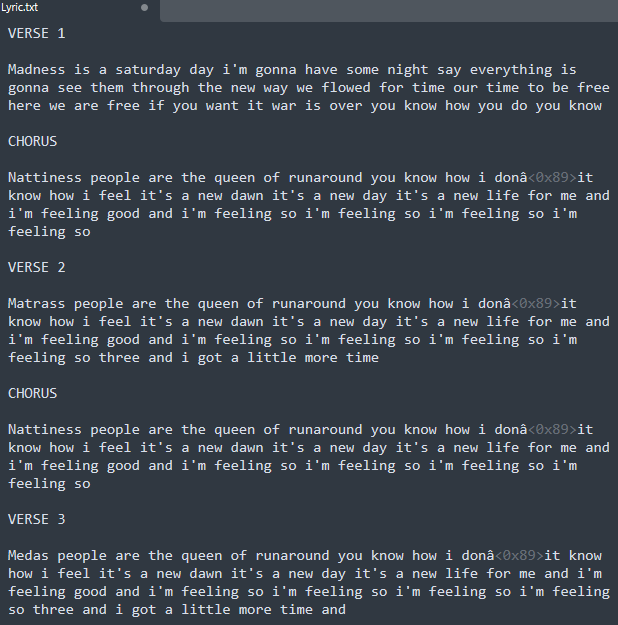
\includegraphics[width=13.5cm]{./Imagenes/Capturas/Textodescargado.png}
			\centering \caption{Texto del archivo descargado.}
		\end{figure}
		
		\item Regenerate Lyrics: Da la posibilidad de generar otra letra de canción con la misma palabra de la primera solicitud.
		
		\begin{figure}[H] 
			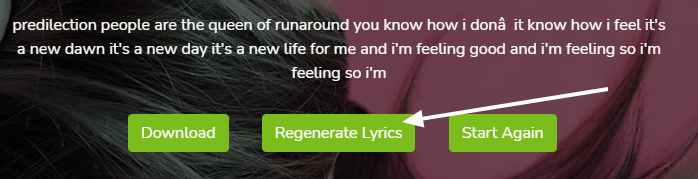
\includegraphics[width=13.5cm]{./Imagenes/Capturas/BotRegen.png}
			\centering \caption{Botón para generar lyric de nuevo.}
		\end{figure}
	
		\begin{figure}[H] 
			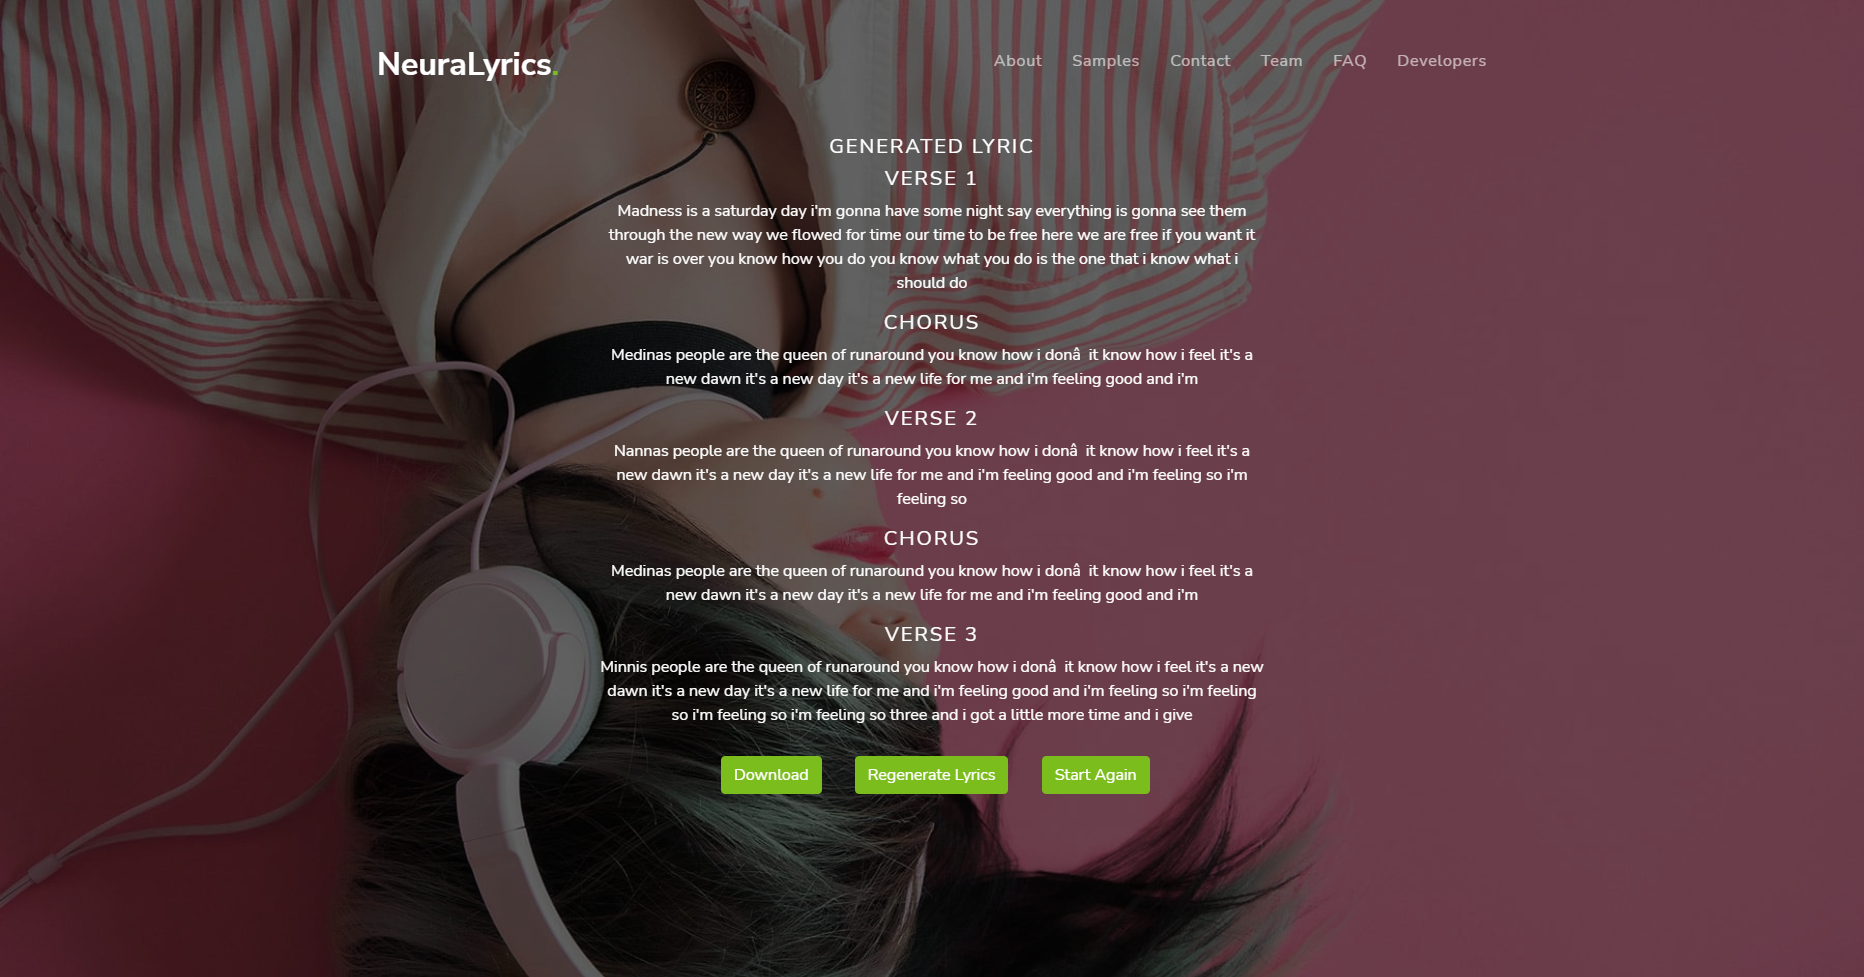
\includegraphics[width=13.5cm]{./Imagenes/Capturas/Regenerate.png}
			\centering \caption{Nueva letra con la misma palabra.}
		\end{figure}
		
		\item Start Again: Lleva a la pantalla anterior para volver a rellenar el campo con la palabra deseada.
		
		\begin{figure}[H] 
			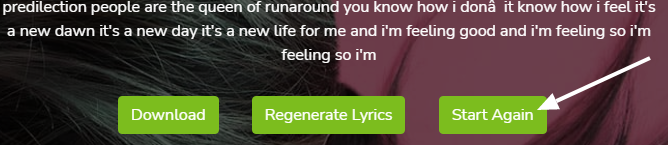
\includegraphics[width=13.5cm]{./Imagenes/Capturas/BotStart.png}
			\centering \caption{Botón para reiniciar el proceso.}
		\end{figure}
	
		\begin{figure}[H] 
			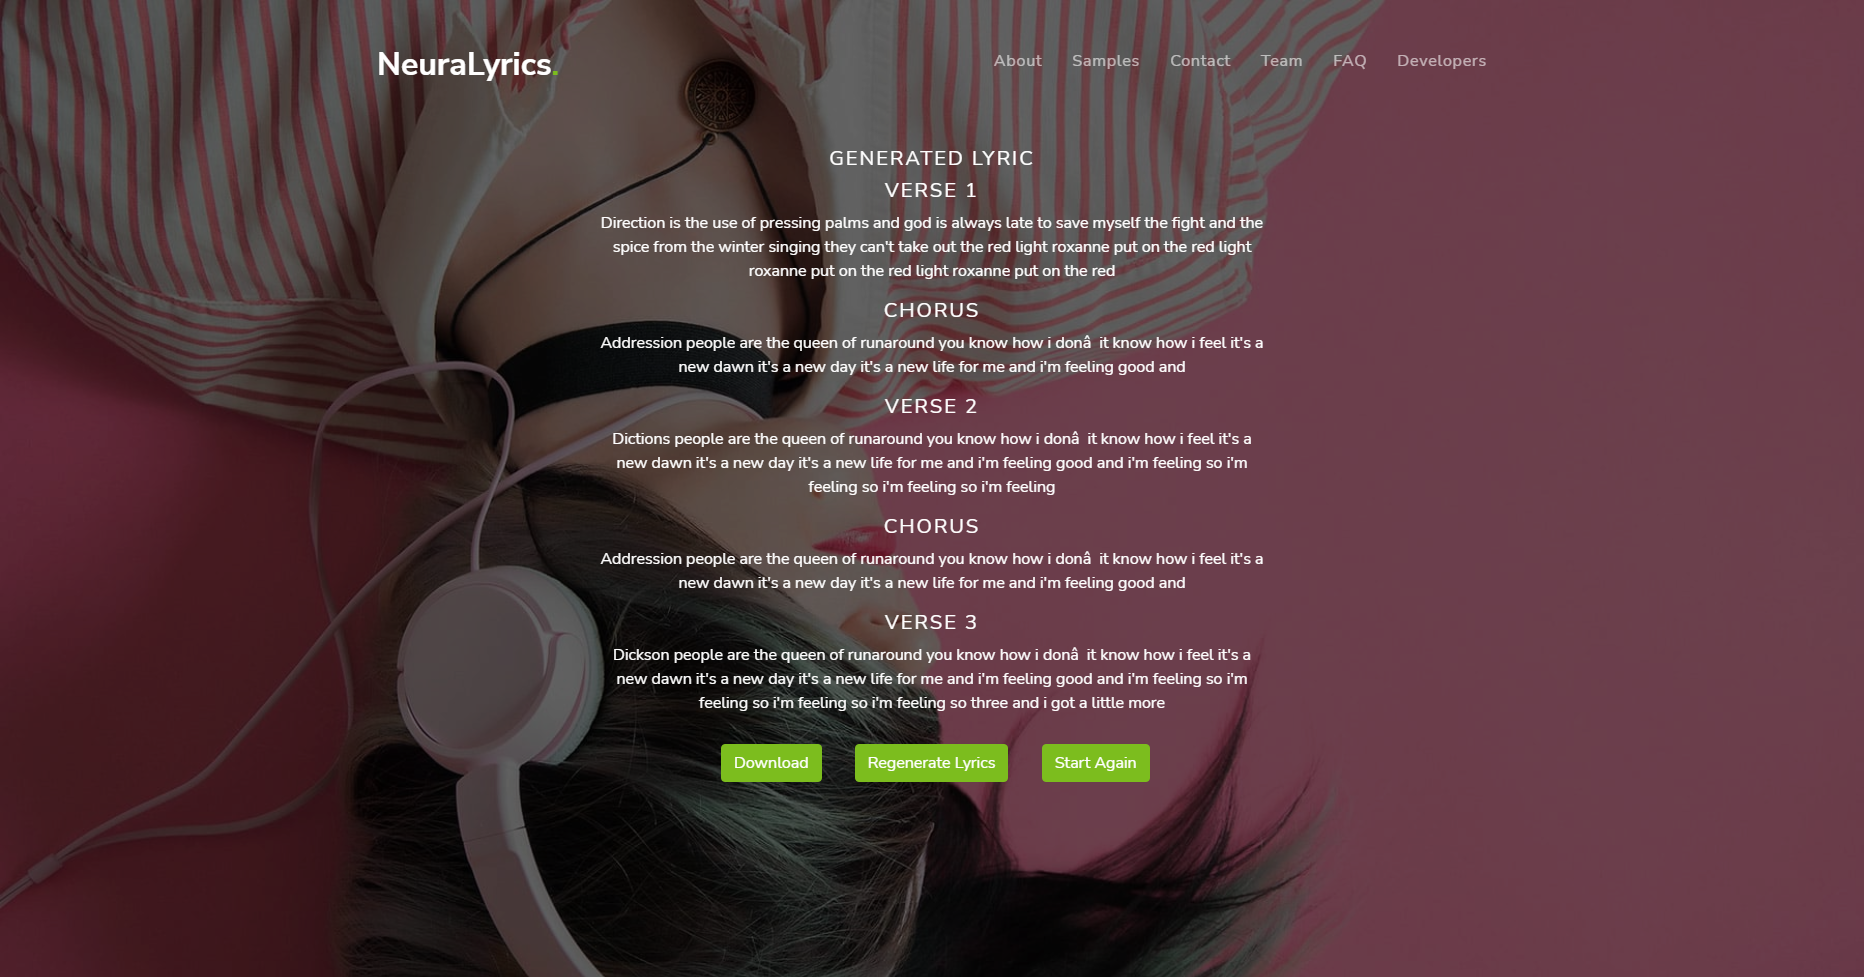
\includegraphics[width=13.5cm]{./Imagenes/Capturas/StartAgain.png}
			\centering \caption{Página con la letra generada a partir de una nueva palabra.}
		\end{figure}
	
	\end{itemize}	

		\section{Pantalla About}
		Esta pantalla presenta información acerca del equipo, objetivos y metas de la aplicación.
		
		\begin{figure}[H] 
			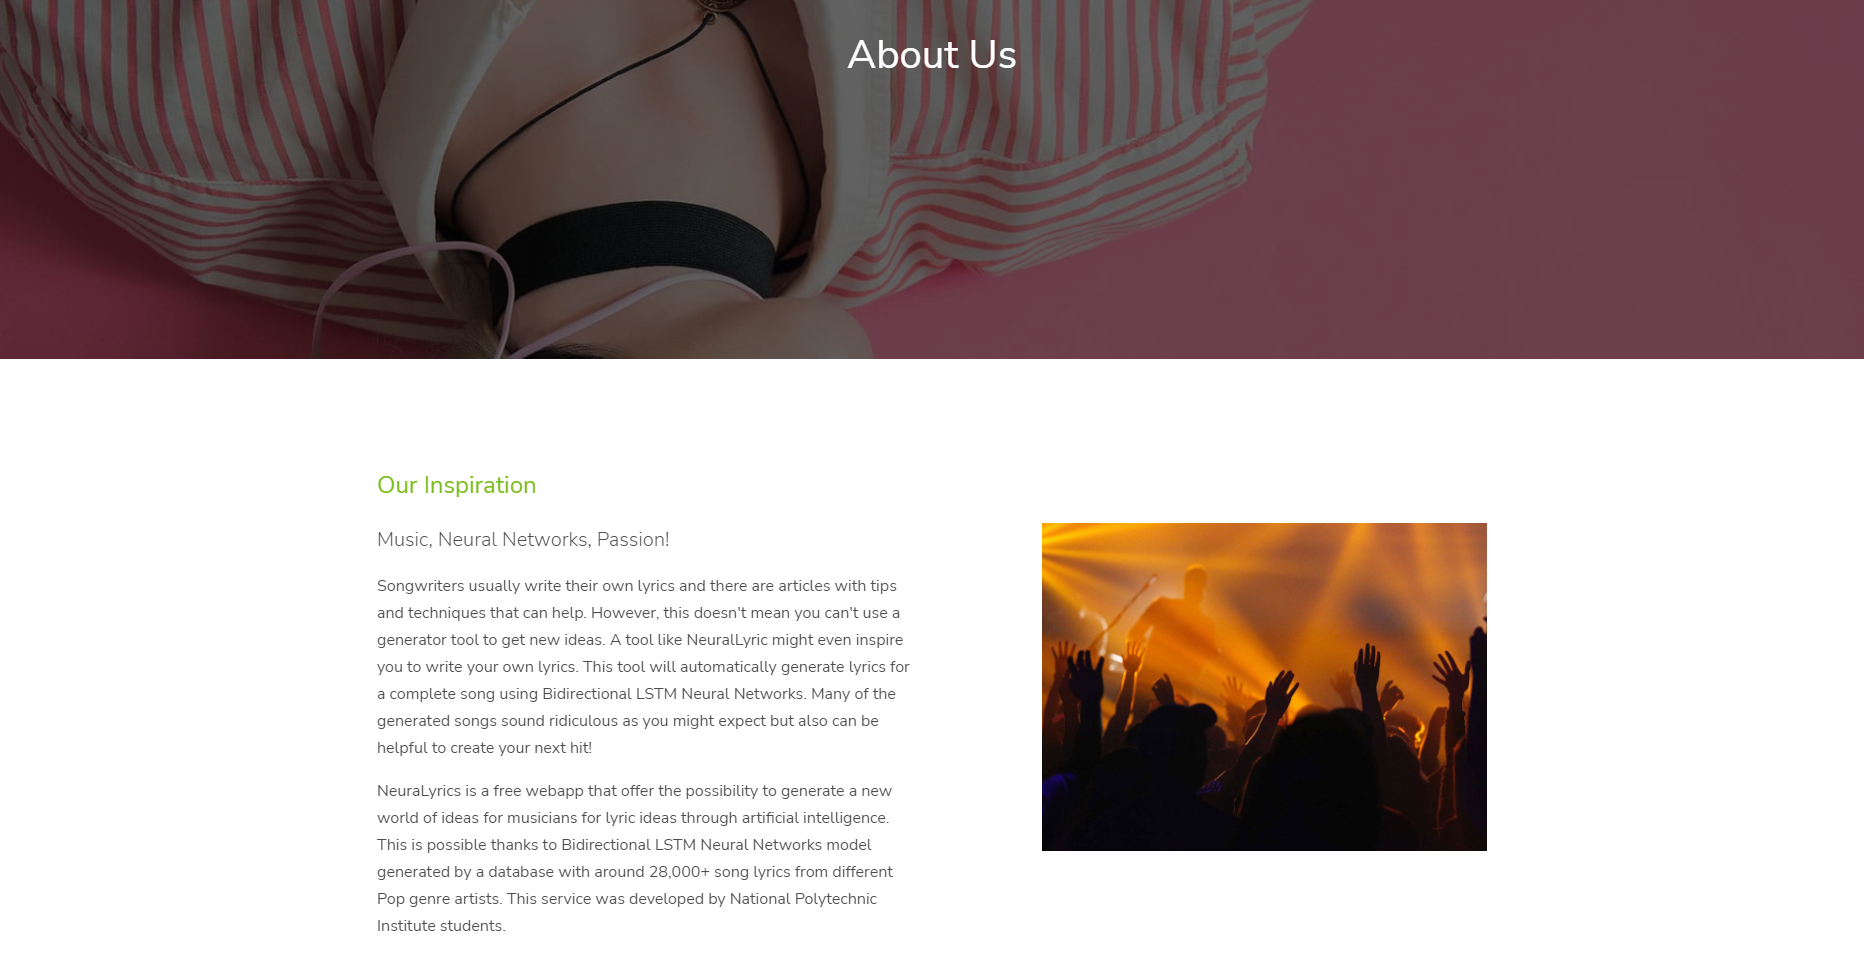
\includegraphics[width=13.5cm]{./Imagenes/Capturas/pabout.png}
			\centering \caption{Pantalla de About.}
		\end{figure}
	
		\section{Pantalla FAQ}
		Pantalla que presenta las preguntas frecuentes que podría tener el usuario antes de tener que contactar a soporte, cuenta con menú desplegable en cada pregunta para que la interfaz se vea más limpia y el usuario no este saturado de texto.
		
		\begin{figure}[H] 
			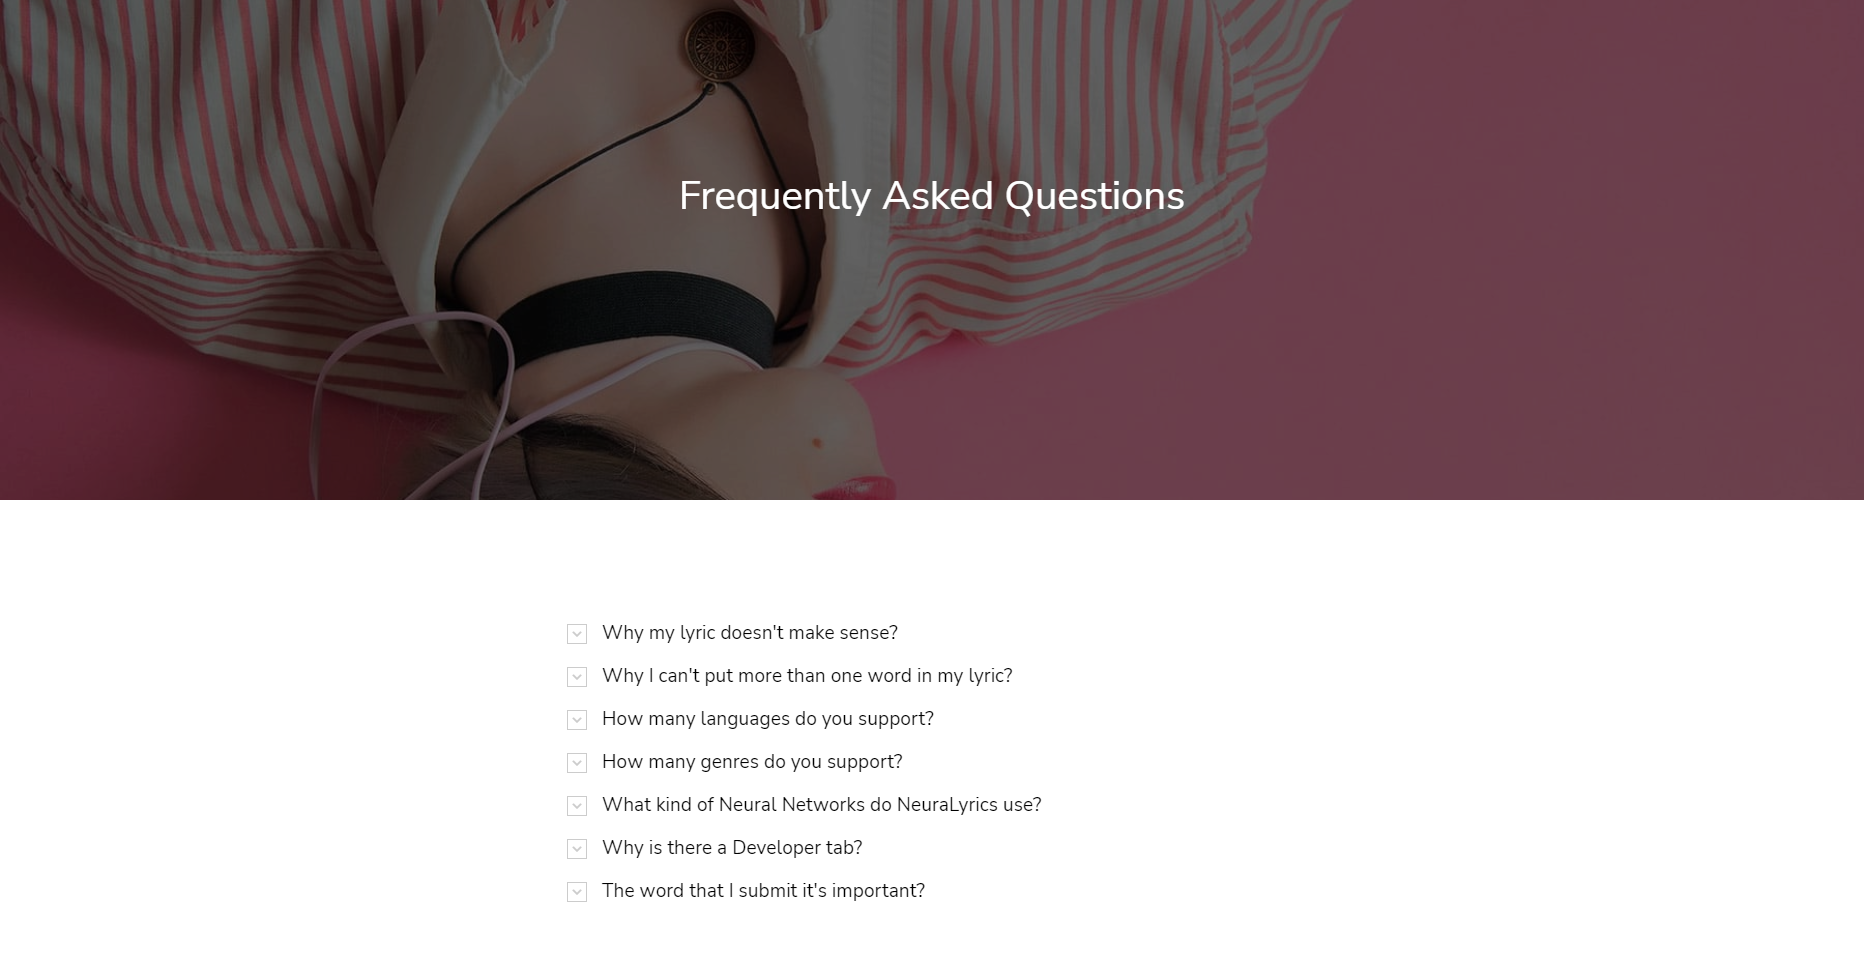
\includegraphics[width=13.5cm]{./Imagenes/Capturas/pfaqclose.png}
			\centering \caption{Pantalla de preguntas frecuentes con el menú oculto, mostrando solo las preguntas.}
		\end{figure}
	
		\begin{figure}[H] 
		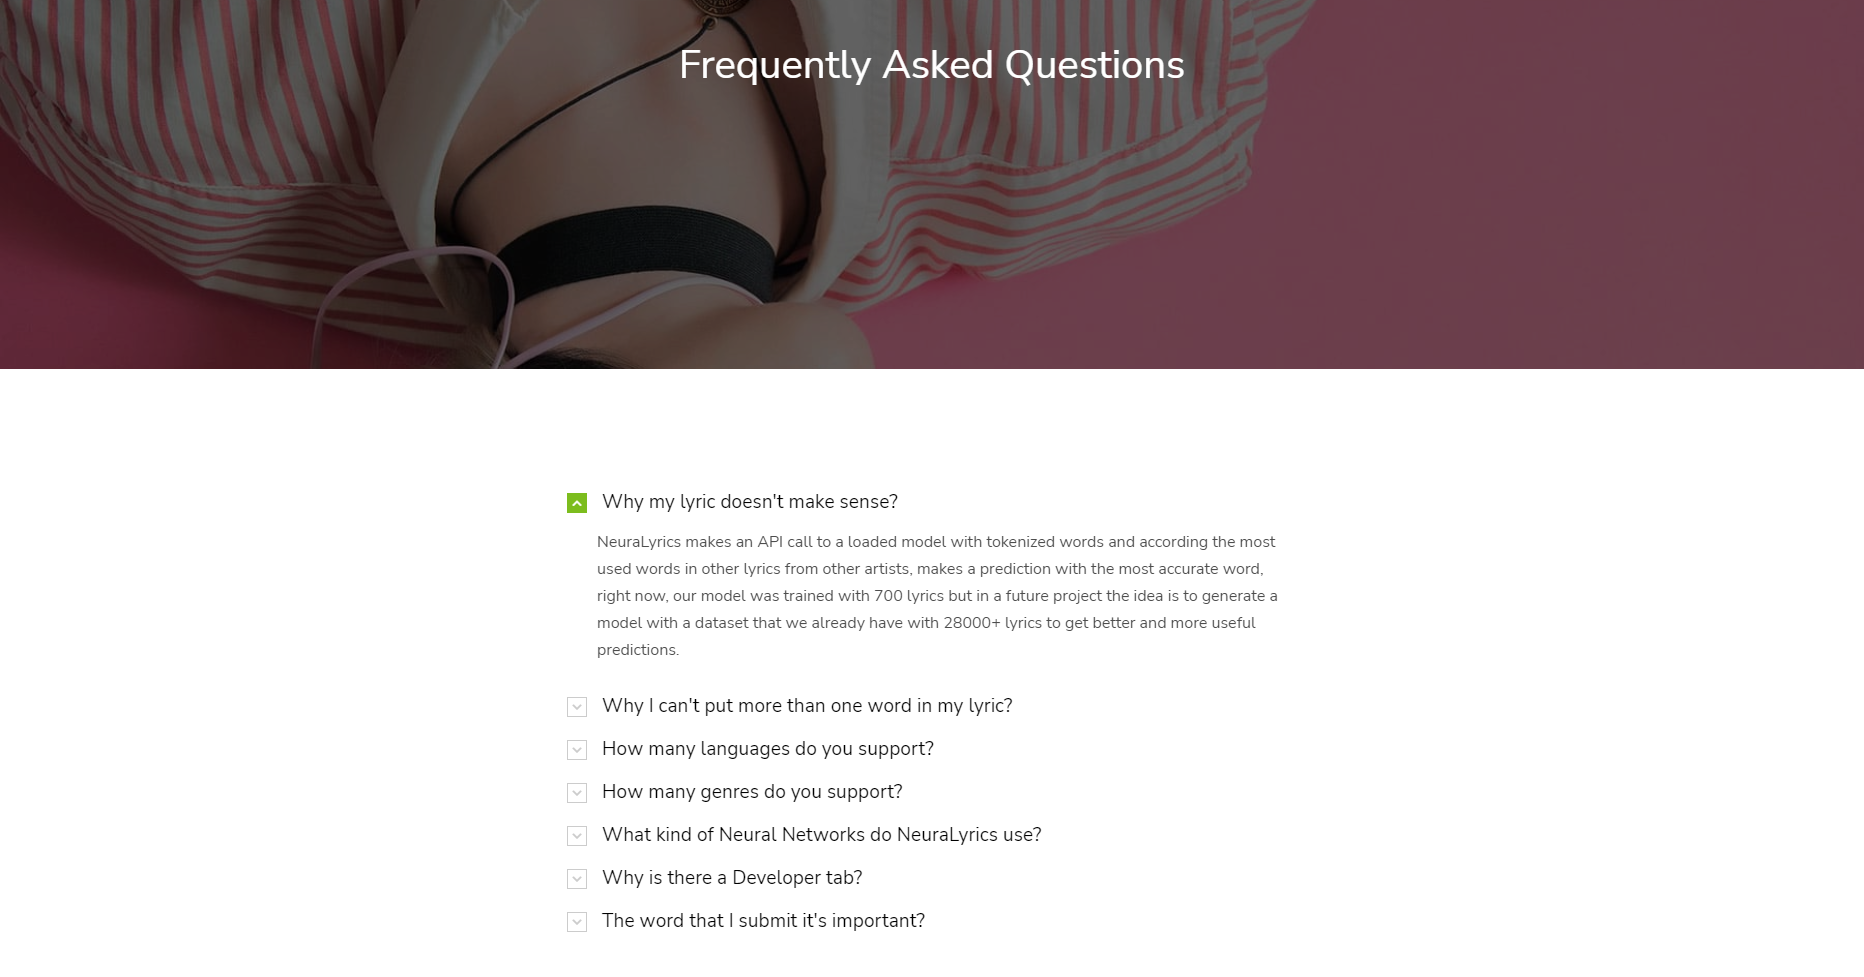
\includegraphics[width=13.5cm]{./Imagenes/Capturas/pfaqopen.png}
		\centering \caption{Pantalla de preguntas frecuentes con el menú desplegado, mostrando preguntas y respuestas.}
		\end{figure}
	
		\section{Pantalla Developers}
		Es una pantalla que muestra la documentación apropiada de la API generada a desarrolladores, en caso de que se requiera implementar llamadas al microservicio creado para poder generar lyrics, el usuario podrá acceder a esta pantalla y revisar los endpoints funcionales con una interfaz amigable para los desarrolladores.
		
		\begin{figure}[H] 
			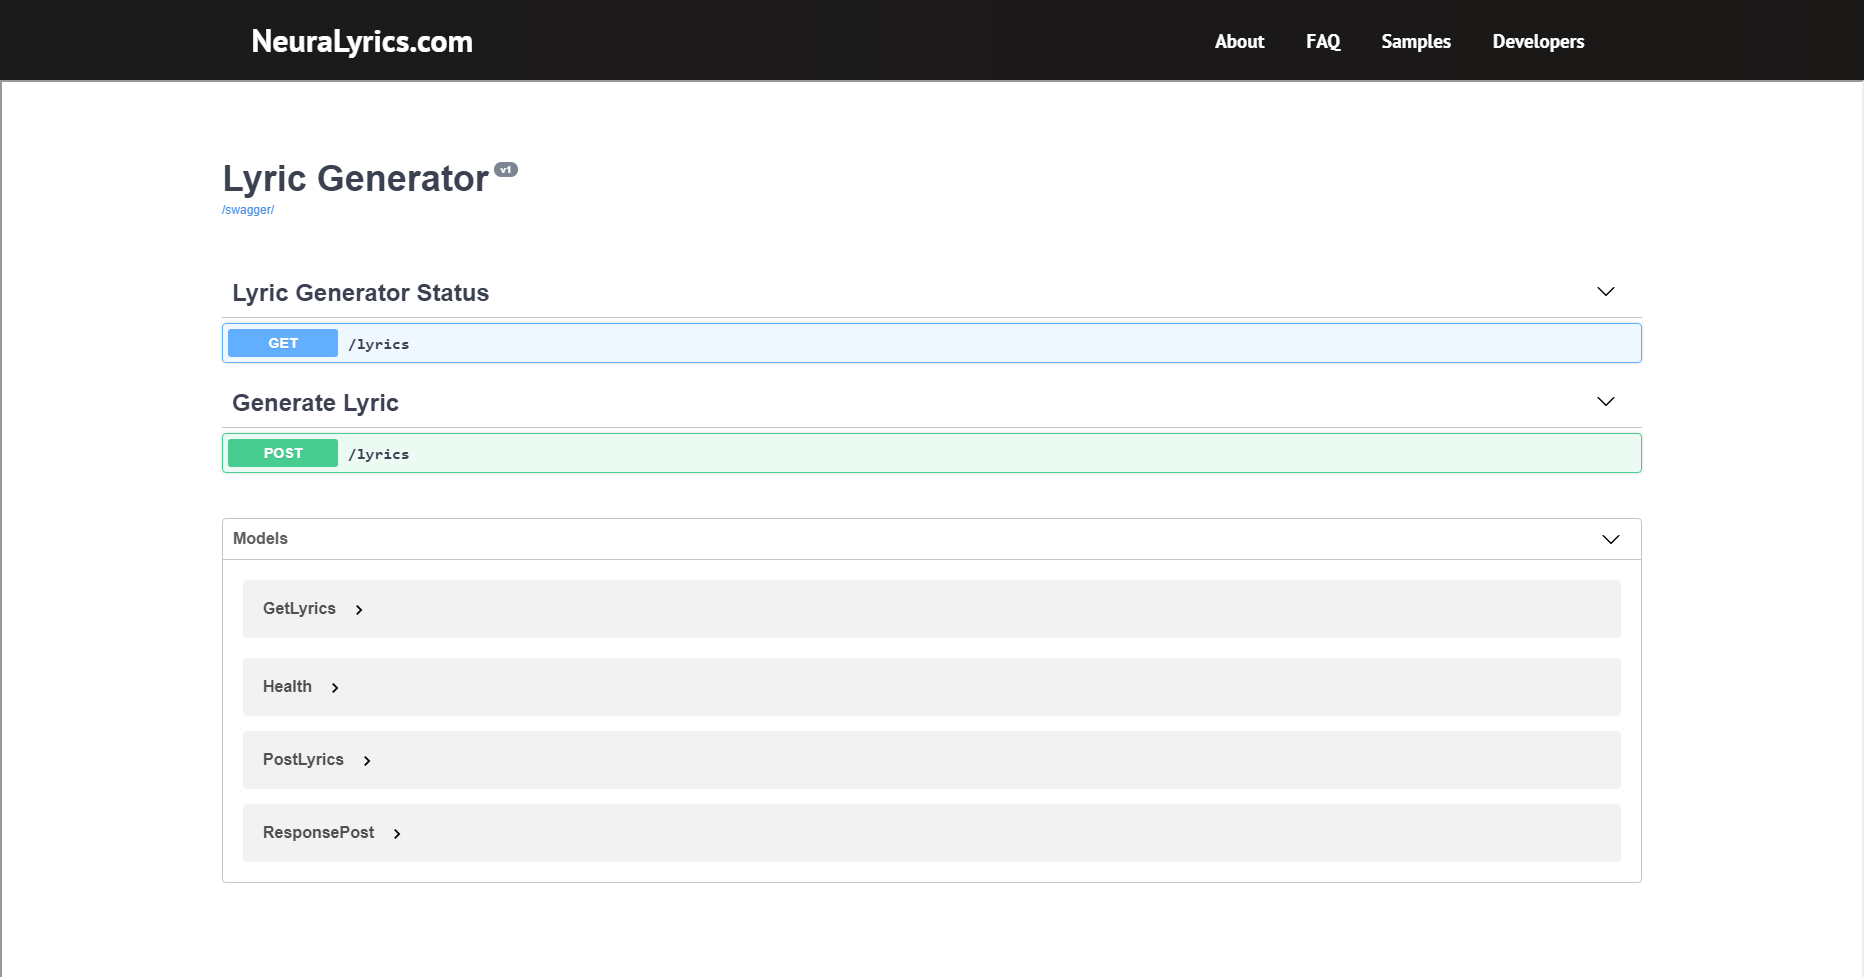
\includegraphics[width=13.5cm]{./Imagenes/Capturas/pdev.png}
			\centering \caption{Pantalla de developers mostrando los endpoints a los que se pueden acceder para llamar al microservicio.}
		\end{figure}
		
		\section{Pantalla Samples}
		Pantalla informativa para mostrar algunos ejemplos sobresalientes generados para que se de una idea del posible resultado al utilizar la aplicación.
		
		\begin{figure}[H] 
			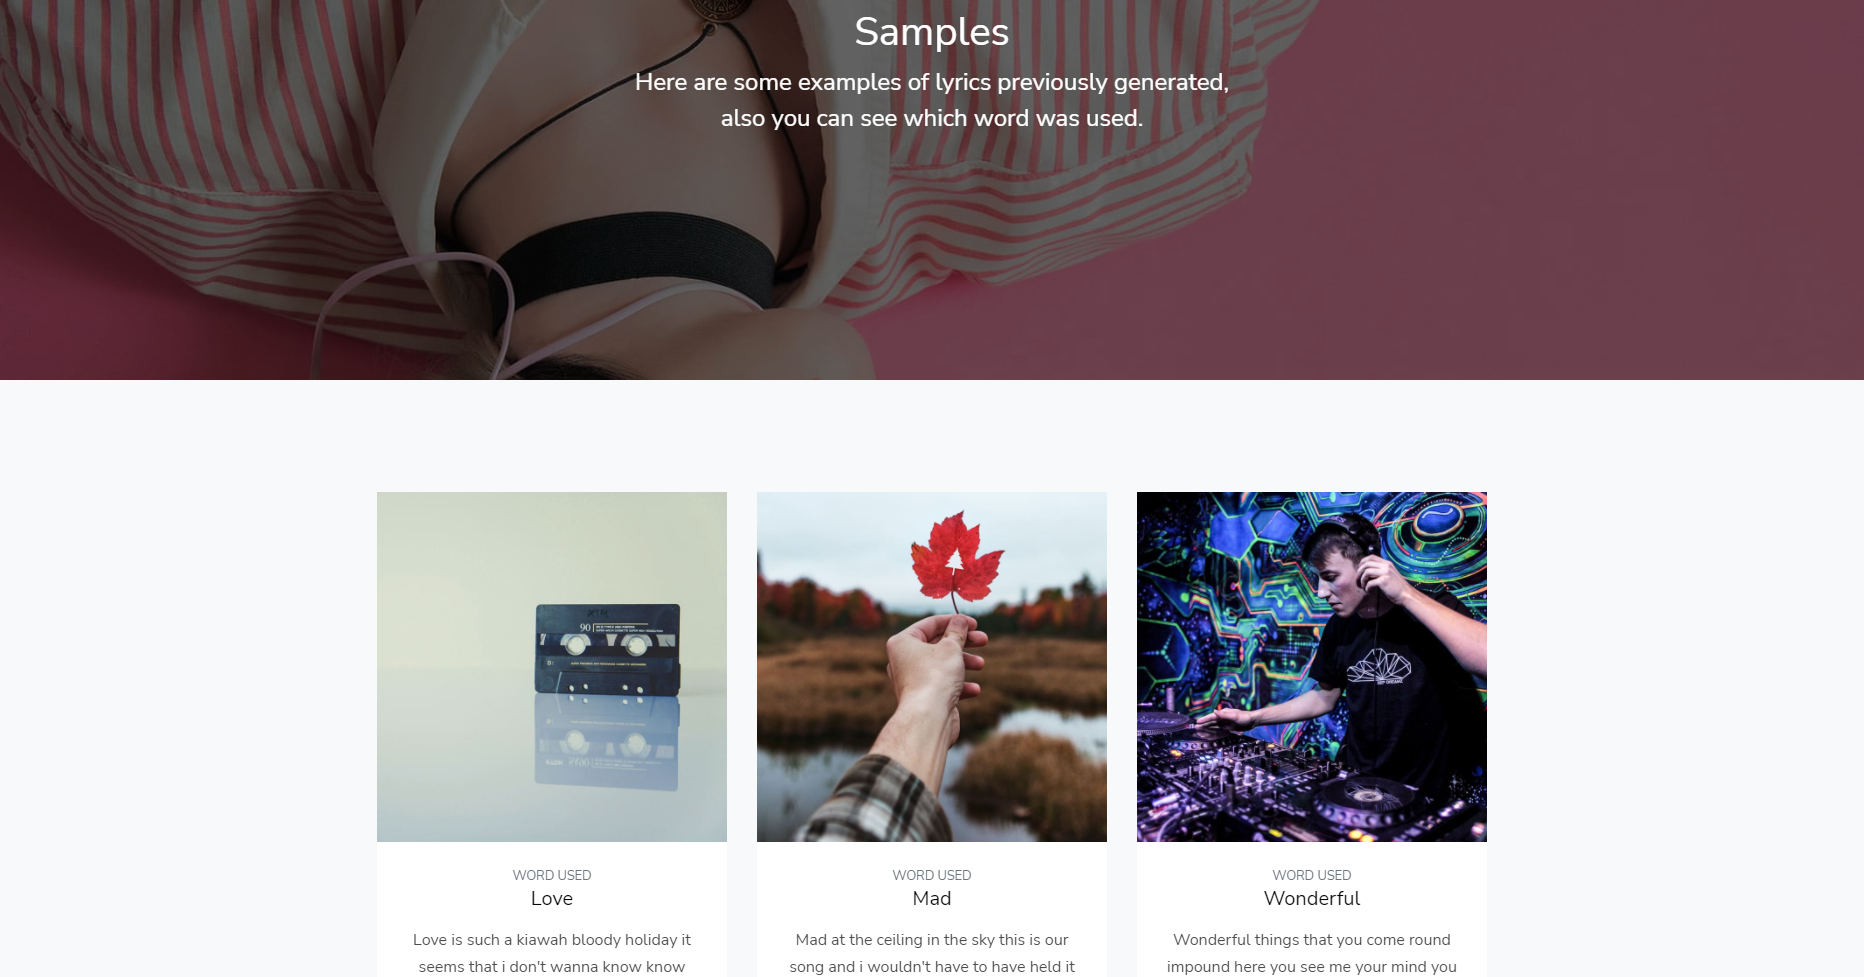
\includegraphics[width=13.5cm]{./Imagenes/Capturas/psamples.png}
			\centering \caption{Pantalla informativa con algunos ejemplos de letras generadas.}
		\end{figure}
	
		\section{Pantalla Contact}
		Para tener contacto directo con los desarrolladores del micro-servicio y la página accediendo a esta pantalla, si se rellena el formulario con los datos de cada campo y dando clic al botón de “Enviar", se establecerá comunicación por medio de correo electrónico a la dirección ttlyrics.escom@gmail.com, que será revisado y contestado personalmente por algún integrante del equipo desarrollador.
		
		\begin{figure}[H] 
			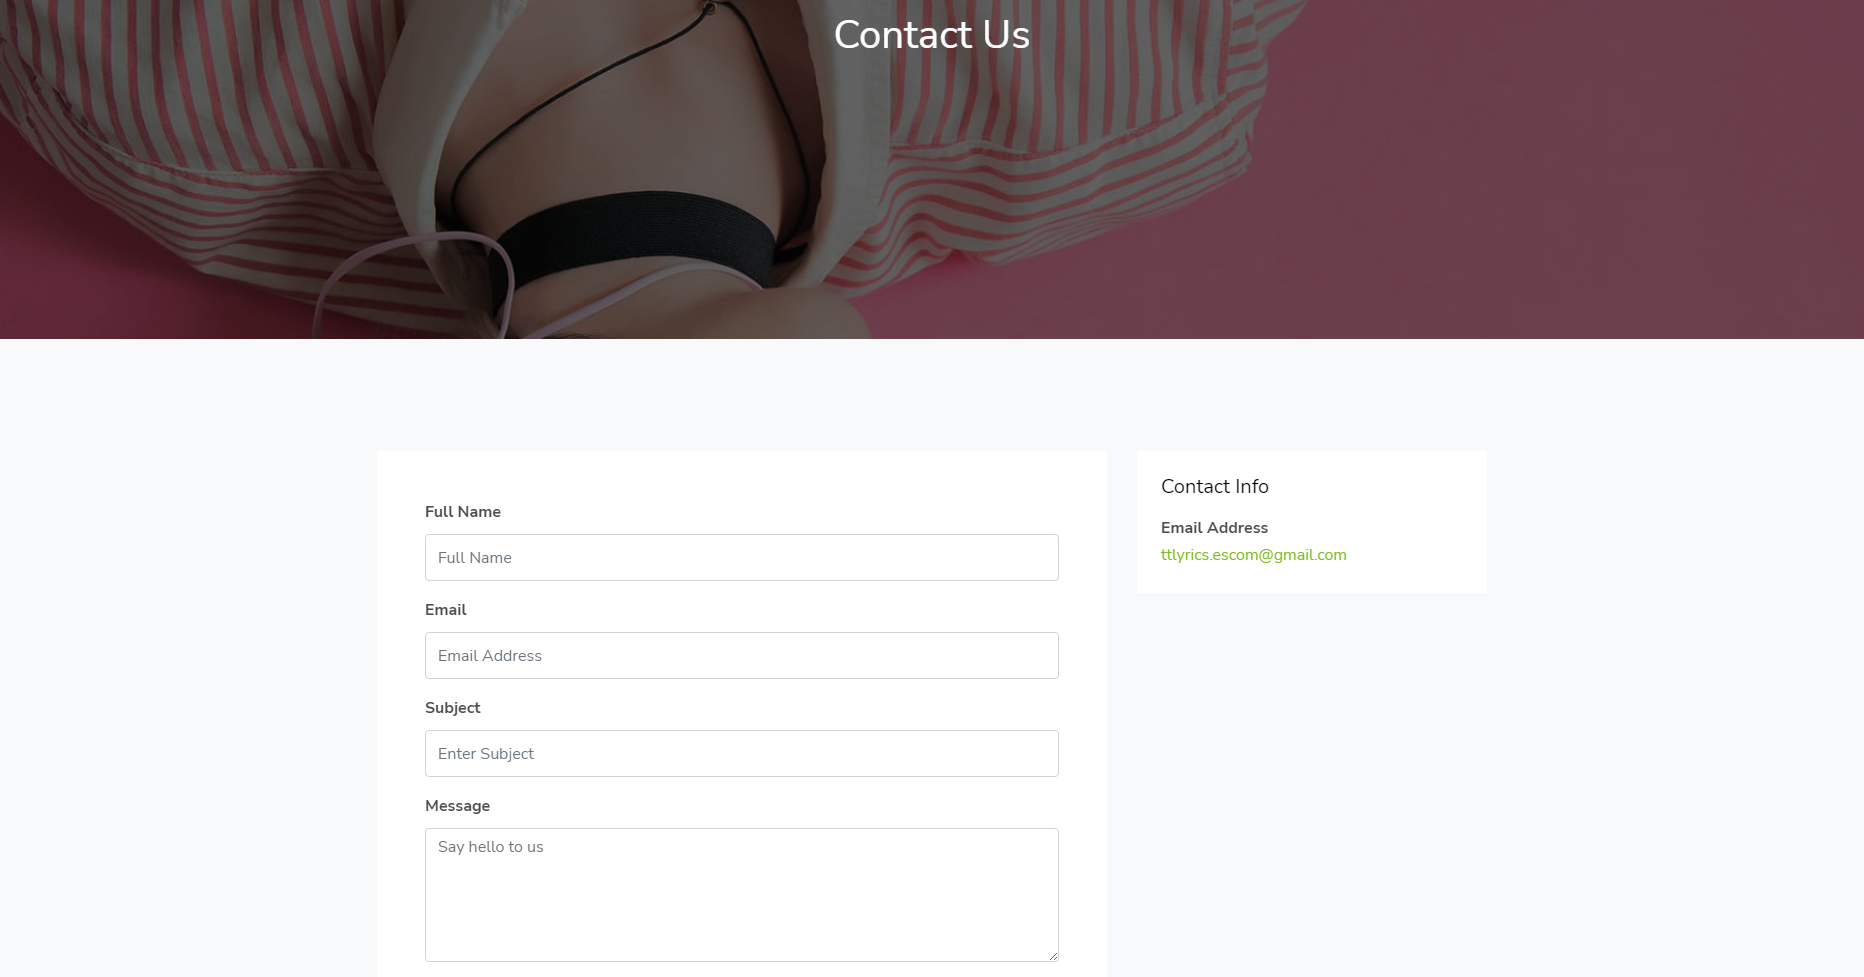
\includegraphics[width=13.5cm]{./Imagenes/Capturas/pcontact.png}
			\centering \caption{Pantalla de contacto.}
		\end{figure}
		
\end{document}